% (c) 2020 Stefan Antonowicz
% Based off of tex found at https://github.com/ludus-leonis/nipajin
% This file is released under Creative Commons
% Attribution-NonCommercial-ShareAlike 4.0 International License.
% Please do not apply other licenses one-way.

\renewcommand{\yggMarvels}{%
  \mychapter{Marvels}{marvels}
}

\renewcommand{\yggMarvelsText}{%



%%%%%%%%%%%%%%%%%%%%%%%%%%%%%%%%%%%%%%%%%%%%
%%% MIRACLE WORKING
%%%%%%%%%%%%%%%%%%%%%%%%%%%%%%%%%%%%%%%%%%%%


\mysection{Miracle Working}{marvels-miracle-working}

\example {

    Faith Dice are used to perform Miracles.  Miracles must be performed on Hallowed Ground (a shrine, church, etc.) dedicated to your Small God, and you must have a \mylink{Holy Symbol}{miracle-holy-relic} \\~
    \\~
    \mybold{Spending} a Faith die means you lose it permanently

}



\mysubsection{Ambrosia}{miracle-ambrosia}

You can create \DICE d4 \UD of Provisions. These \UD can be combined into a single \UD (see "Adding and Splitting Usage Dice" in the Arbiter's Miscellania section of hte core rules). These Provisions can be stored for use later, but it also particularly nourishes the faithful.  During the working of the Miracle, up to \DICE disciples of the Small God can partake of the Ambrosia and gain +1 Faith Die (the miracle worker cannot gain this benefit). Disciples partaking of the meal do not affect the \UD produced in any way.

\cbreak

\mysubsection{Covenant}{miracle-covenant}

You seal a bargain between yourself (the Suzerain) and another (the Vassal) by awarding your Small God temporary control over your collective *noumenon* (this means that the Unhallowed can't be held to a Covenant).  A Covenant has to be given freely, but can be compelled by other factors (like a dagger to the throat).

Roll a number of \DICE equal to the \LVL of the Vassal and gain the following effects:

\mybullet { 
  \item Immediately spend a single Faith die.  You can give and take Faith from the Vassal as if they were a disciple (see the Mystic Virtue "Fishers of Men" in the core rules).
  \item You always know where your Vassal is and feel any strong emotions (lust, hatred, etc) or  physical extremes ("he's somewhere very, very cold") they might be enduring
  \item You can't directly harm your Vassal (though you can command others to do so); your Vassal isn't likewise constrained
  \item Your Vassal is immediately converted to the worship of your Small God
  \item Your Vassal barely needs sleep, and eats and drinks sparingly (roll Provisions \UD twice and take the higher roll).
  \item Your Vassal is affected as if they were under the effects of \mylink{Tongues of Fire}{miracle-tongues-of-fire} at all times
  \item Your Vassal gains +\SUMDICE points of "holy armor".  Damage is subtracted from this total first before it is applied to Armor, Grit, etc.  It can't be healed, but it can be restored during a Vacation by worshipping at a shrine, church, etc. dedicated to your Small God
}

You and your Vassal can only have a single Covenant at any time.  The Covenant can be broken by one of you having a Crisis of Faith; the death of you or your Vassal; or by mutual, peaceful agreement.

\newpage

\mysubsection{Crusade}{miracle-crusade}

Transforms your Vassal into a Paladin of the Faith.

  \begin{center}
  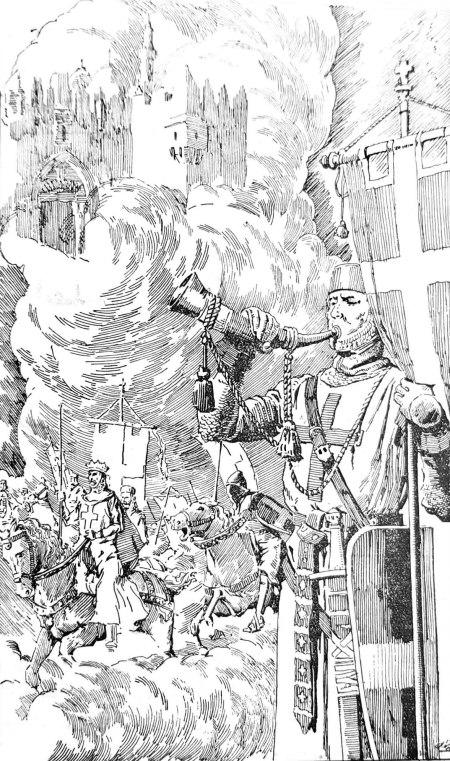
\includegraphics[scale=.5]{Crusade}
  \end{center}


Roll a number of \DICE equal to the \LVL x2 of the Vassal and gain the following effects (in addition to the benefits of being a Vassal):

\mybullet { 
  \item Your Vassal can use their Faith as if they were a Sellsword's Deed Die.  If they're already a Sellsword, they now have 2 Deed Dice they can roll together or separately.
  \item Your Vassal can gain Faith on their own (they don't need you to give it to them) up to a [max] of 4 
  \item Your Vassal can cast any of the Seven Sacraments using their *Faith* Dice (see the Mystic Virtue "Gift of Grace" in the core rules)
}

You now have to name a \myital{jihad} important to your Small God: "wipe out the infidels of the Crawling Chaos", for example, or "bring the fingerbone of St. Sebastien to the reliquary in the Howling Wastes".  Similar to a Geas, any day not spent in the furtherance of the cause of the Crusade will lose your Vassal a single Faith die.  It's important to note that if your Vassal should lose all their Faith and suffer a Crisis of Faith, the Crusade has failed and the Covenant is broken.



\mysubsection{Golem}{miracle-golem}

A golem is a mortal-like figure, brought to life through magic.  Creating a golem requires gold for materials and effort in addition to spending Faith Dice:

\mytable{X c c} {
  \thead{Type} & \thead{\COST} & \thead{Faith Dice} \\
} {
  Paper  & 50\AU  & 8 \\
  Glass  & 100\AU  & 10 \\
  Wood  & 500\AU  & 12 \\
  Clay  & 1,000\AU  & 14 \\
}

Golems requires a *shem* - a slip of paper with a magical rune written on it through the miracle of the \mylink{Holy Writ}{miracle-holy-writ}.

Golems are completely obedient to you and respectful of other followers of your Small God; presenting a Holy Symbol of your Small God is enough to keep them at bay, but only you can command them.  If you should die, the golem will continue performing your last command in perpetuity.

\mybold{Golems are immune to magic of any kind - including arcana and magical weapons.}

\myhighlight{Paper Golem}{miracle-paper-golem}

Paper golems are small (less than 100cm tall) creatures created for menial work to fetch and carry.  They can carry a single Significant Item provided it doesn't weight more than 5kg (or a number of Insignificant Items up to 5kg).  Paper golems can "fly" on gusts of wind (similar to how a chicken can "fly") and walk and run as fast as a small child.  Paper golems record everything they see.  At any time, you can ask them a single question ("what was it you saw when you were in the Baron's chamber?", for example) and the golem will flatten itself into a scroll upon which is written what it "saw". The Golem remains a scroll forever more, with the symbol of the Small God embossed on the bottom of the scroll.  These embossed scrolls are very, very difficult to counterfeit - and the price if you get caught is high, as it would bring down the wrath of the entire church of your Small God.

Paper Golems are immediately destroyed by (non-magical) fire

\myhighlight{Glass Golem}{miracle-glass-golem}

Glass golems are 2m tall automatons filled with pungeant herbs and combustibles called "smokes".  You determine the type of smoke at the point of creation. Glass golems immediately explode when dealt a forcible blow - a hit with a weapon, a fall from a height greater than 3m, etc.  The effect of exploding a Glass Golem deals d6 damage to everything Nearby (Save negates) as well as the following effects:

1. Smoke of Chaos:  every Nearby creature is Befuddled and Enraged (1-3 on a d6) or Afraid (4-6 on a d6)
2. Smoke of Heroes:  every Nearby Ally receives a Blessing, and are immune to fear of any kind - but they can't retreat.
3. Smoke of the Holy: explodes to create Hallowed Ground in a circle 15m in radius; this can be used to create Hallowed Earth, or dispel Unhallowed Earth (if the radius is less than 15m).  Unhallowed creatures Close to the explosion are thrown 15m Nearby (treat as Falling Damage).
4. Smoke of Medicines: every Nearby Ally heals to \MAX Flesh and Grit

the smoke persists for Minutes, but can be dispersed by wind.  You are not limited to these options; they should discuss with the Arbiter if they wish to go a different way.


\myhighlight{Wood Golem}{miracle-wood-golem}

Wood golems are 3m docile, hulking, tree-like creatures possessing great strength. They are able to carry up to 50 Significant Items in their branches weighing up to 1,000kg total.  They can successfully break down non-magical doors, bend iron bars, and perform other feats of strength on a 4-in-6 (this number can be adjusted at the Arbiter's discretion).  They walk at a slow, shuffling gate (d4 \MD)

Wood golems will never attempt to defend themselves.  They can take up to 50 points of damage - Chopping weapons deal double-damage, and fire deals triple-damage.  They will glad and mindlessly stand wherever you demand: in front of a doorway, in the middle of a fire, or charging dumbly into a group of Monsters.

\myhighlight{Clay Golem}{miracle-clay-golem}

Clay golems are giant (4m tall) faceless creatures created to protect or guard an area.  You must tell them what they must guard at the moment of their creation, and they cannot stray further than 100m from that spot.  The spot they guard must be Hallowed, and if this ever ceases to be they will immediately crumble to dust.

Clay golems house the *noumenon* of a Vassal or Paladin of their Maker (see \mylink{Covenant}{miracle-covenant}) and \mylink{Crusade}{miracle-crusade}.  Your Vassal is ritually slain, and their blood is mixed with sacred earth and fire to create the clay giant. Your Vassal does not need to be a willing sacrifice, but remember you can't directly harm your Vassal.  The Clay Golem has all of the memories, skills, saves, and abilities of their Mortal form (including Deed Dice, spell casting, etc.) and Grit, Flesh, etc.  They have a Soak: 2 and do 2d8 damage (2 Close).  They are immune to spells of the Mind paradigm, backstab, surprise, and toxins. They cannot speak and are unswervingly obedient.

Clay golems can house the spirits of willing heroes (paladins who wish to protect the temple forever) or with those of unwilling enemies (forced to guard a forgotten hallway, or the temple of a heretic Small God).  When slain, the *noumenon* of the deceased do not travel to the Isle of the Dead.  None know what happens to their souls. 


\mysubsection{Hallowed Ground}{miracle-hallowed-ground}

You can either desecrate \mylink{Unhallowed Earth}{occultism-unhallowed-earth}, or create Hallowed Ground for performing miracles, somewhere within \DICE km of you.  You create / desecrate an area \DICE meters in diameter.  If you're attempting to desecrate Unhallowed Earth, the diameter must be equal to or exceed the area of the Unhallowed Earth.  You must create a \mylink{Holy Write}{miracle-holy-writ} that will be consumed during the miracle; this Holy Writ identifies the Hallowed Ground as "belonging" to your Small God.  Another Mystic will know the size of the Hallowed Ground just by looking at it, but only other Mystics who worship your Small God will know which God the Hallowed Ground belongs to.


Hallowed Ground provides the following benefits:

\mylist {
  \item no Unseelie or Unhallowed creature may enter Hallowed Ground
  \item all Mortals inside the radius of the Hallowed Ground can immediately end a Markovian effect
  \item all Mystics on Hallowed Ground may ignore the negative effect of a Failure when using their Grace (that is, they may keep their Grace die even if they roll a 1 or a 2).
}

This miracle is the only one that does {not} require Hallowed Ground to perform.

\mysubsection{Holy Relic}{miracle-holy-relic}

A repository for Faith.  You can spend \DICE Faith and place them in the relic at the time of its creation.  This Faith can be used by other Mystics of your Small God (as well as yourself).  The relic itself must be something "special" - a fingerbone of a Saint, a shroud, etc.  - at the Arbiter's discretion.  The more powerful the relic, the more Faith can be placed inside of it.

The Miracle of the Holy Relic is used to create \mylink{Holy Symbols}{mystics-liturgies}.  The symbol must be what is indicated under your Small God.  A Holy Symbol only requires you to spend a single Faith \POOL

  \begin{center}
  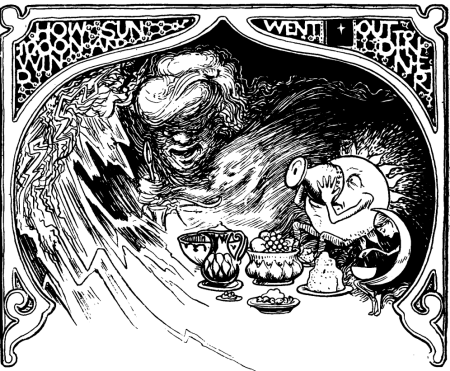
\includegraphics[scale=.5]{Miracle_1}
  \end{center}


\mysubsection{Holy Water}{miracle-holy-water}

You can spend \DICE Faith to create \DICE d4 \UD of Holy Water.  These \UD can be combined into a single \UD (see "Adding and Splitting Usage Dice" in the Arbiter's Miscellania section of hte core rules). For each Faith Die spent, you must spend 25\AG in materials.

\mysubsection{Holy Writ}{miracle-holy-writ}

The word and the law of your Small God, written as seven sacred words known only to the faithful.  Only you and other members of your faith can see the words; to others, they look like random squiggles, strange designs, or "primitive" carvings.  Contained in the seven words is the Mystic who performed the Miracle, but you will need to make a successful Skill: Lore check to identify them unless you know them personally.   The Holy Writ only requires you to spend a single Faith \POOL


\mysubsection{Incorruptibility}{miracle-incorruptibility}

This Miracle can be performed on a corpse to stop a body from rotting.  The length of time depends on the number of Faith dice invested:  1 [die]: \SUMDICE Days; 2-5 \DICE: \SUMDICE Weeks; 6-9 \DICE: \SUMDICE Years; 10+ dice: \SUMDICE Centuries.  So long as the body remains on Hallowed ground, it does not decay in any way and cannot be targeted with any spells from the Necromancy paradigm.  If the body is removed from Hallowed ground, it will begin to decay as normal.

\mysubsection{Proselytize}{miracle-proselytize}

You can attempt to convert others to the faith of your Small God, or give willing congregants instruction in the ways of your religion.  

You can spend 1 Faith die on as many Mortals (not Unseelie) as you choose, provided they are not Mystics who follow a different Small God.

The effects vary depending on whether the congregant is willing, apathetic, or unwilling

\mylist {

\item Willing:  you give one of your Faith Die to the worshiper
\item Apathetic:  roll the Faith \POOL; on a failure, the die is lost.  On success you have converted them - instead of giving your Faith Die to them, they gain one of their own
\item Unwilling:  the congregant gets a Save vs Doom.  If they succeed, you lose 2 Faith Die (the original you tried to give them, plus one other).  If they fail, roll as "Apathetic" above - if you succeed in converting them, you gain +1 Faith
}

Worshipers who have a Faith Die from you become your Disciple (see the Mystic Virtue "Fishers of Men" in the core rules).

\mysubsection{Sacred Mass}{miracle-sacred-mass}

You can perform a sacred ceremony for \SUMDICE others (excluding yourself).  Non-Mystics who indulge in a Sacred Mass are Blessed for the remainder of the Session (or for the next Session at the Arbiter's discretion).  If you are a Mysic of a different Small God then the miracle worker and partake in the Mass, you lose 2 Faith Die.  If you are the miracle worker, or a Mystic of the same Small God, you gain 1 Faith Die for every 10 people participating up to your \MAX.



\mysubsection{Sin Eating}{miracle-sin-eating}

You can heal up to \DICE serious and non-serious Spirit Wounds on yourself or others

\cbreak

\mysubsection{Tongues of Fire}{miracle-tongues-of-fire}

Up to \SUMDICE people other than the Miracle Worker are affected.  Recipients of Tongues of Fire can speak (but not read) any Language they choose at will, and can command a single creature once per Session (see below).  The recipient can never lie while under the effects of Tongues of Flame.  Unwilling creatures get a Save.  This miracle lasts only for the Session (unless provided by Covenant)


\MYSTERY [
  Name= Command,
  Link=miracle-command,
  Paradigm=Mind,
  Save=Y,
  Duration=0 ,
  Counter= n/a  ,
  Keywords=None ,
  Target=Nearby creature
]

You shout a \DICE word command to the target, who must then carry it out if the fail a Save.  If the command would last more than a single Moment, the target gets a new Save at the beginning of each Moment.


%%%%%%%%%%%%%%%%%%%%%%%%%%%%%%%%%%%%%%%%%%%%
%%% OCCULTISM
%%%%%%%%%%%%%%%%%%%%%%%%%%%%%%%%%%%%%%%%%%%%

\newpage


\mysection{Occultism}{marvels-occultism}


Cunning is required to practice the observances and ceremonies that make up Occultism.   Occultism must be practiced on \mylink{Unhallowed Earth}{occultism-unhallowed-earth}.

\OCCULT[
  Name=Barghest,
  Link=occultism-barghest,
  Success=10+,
  Cost=66\AG (plus see below)
]

You summon a spectral black dog (a harbinger of death and misfortune) to torment a single person for [Cunning] days.  You must whisper the birth name of the victim to the spectre; upon hearing it, the black dog will seek the victim out, traveling up to [Cunning]x100km a night to find them.  The barghest can only travel at night, and disappears at the first light of the rising sun.  The dog can see invisible or hidden creatures and will unerringly find the target provided they are within distance of the casting of the ritual.

Once found, the barghest will appear to the victim once every night.  The victim is permitted a Save vs Doom when they see the Barghest; if they fail, they suffer the curse of the Barghest until it appears again at sunset.  Pooka are immune to Barghests, and if the victim is in a Band with the Pooka, they get two Saves.

If the victim fails their save, the suffer the following maledictions:
- they automatically "take a 1" on Luck checks
- they can't heal Grit
- all \RO and \RB tests suffer a -4 penalty (excluding their Save vs Doom against the Barghest the following night)

The ritual requires a dog (your familiar is fine); an item belonging to the victim; and 66\AG in supplies.  No harm comes to the dog, but the spectral figure will resemble him or her if examined closely

\cbreak

\OCCULT[
  Name=Bind Familiar,
  Link=occultism-bind-familiar,
  Success=5+,
  Cost=666\FE
]

Your familiar is a supernatural creature bound to your soul.  They can be summoned and dismissed at will: they'll appear from a shadow (cat) or sewer grate (rat) or fly in through a window (raven), and they'll leave roughly the same way.  Familiars are Unhallowed, and grant you +1 Cunning if they're with you when you practice Occultism.  

The strength of your familiar depends on the number of [Cunning] you invest when you summon them.  They can be sent on missions up to [Cunning]km away. You can see what they see and hear what they hear for as long as you Concentrate. You also can remember things your familiar remembers (so you could send them on a spying mission and later "remember" what they saw). You can cast Charms through your familiar if you desire.

If your familiar is Close or Nearby, you can communicate verbally with them, though you cannot use words greater than 1 syllable.  You communicate in a language all your own that no one else understands.  They can follow simple instructions ("get the key on the desk", "chew through these ropes", "spy on that man") but not more complex ones ("pick the lock").  Your familiar can't talk.

Familiars have [Cunning] Health.  If you have the Aura Virtue, you can shield them with your Mojo the same way you shield yourself, but you can roll your Mojo as many times as you want (while you have it, anyway) to protect them.  If they're attacked and they survive, they immediately dismiss themselves and won't return for the rest of the Session. If your Familiar dies, you must travel Widdershins before you can summon another.  

Familiars are themselves immune to spells from the Mind paradigm, but if a Mind spell is cast on them you need to Save or be affected as if the spell targeted you.

Finally, you can place a Malison on your familiar (see the ritual below).  In the event of your death, the familiar will stay with your body until someone attempts to disturb your corpse.  At that point, it will deliver the malison etched upon its skin, and dismiss itself for good.

When you summon your familiar, roll below (or discuss with the Arbiter if you want to choose), or make something up.  You can only have 1 familiar at a time.



\myhighlight{Familiars}{occultism-familiars}

  \mytable{l X}{
    \thead{d6} & \thead{Familiar}\\
  }{
    1 & Cat \\
    2 & Dog \\
    3 & Rat \\
    4 & Toad \\
    5 & Raven \\
    6 & Exotic (roll below) \\
  }  

  \mytable{l X}{
    \thead{d6} & \thead{Familiar}\\
  }{
    1 & The severed hands of a condemned man  \\
    2 &  A pet rock \\
    3 & A floating Fist-Sized Crystal Tesseract  \\
    4 & A doll made of rags and straw \\
    5 &  Miniature, horribly deformed homunculus resembling you \\
    6 & An intelligent moss \\
  }  

  \begin{center}
  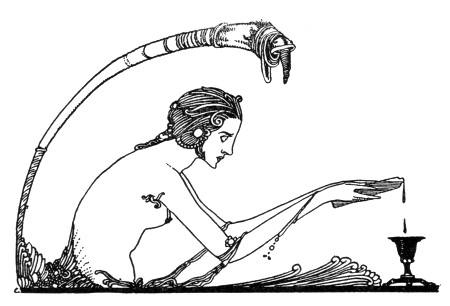
\includegraphics[scale=.5]{Occult_1}
  \end{center}


\OCCULT[
  Name=Create Juju,
  Link=occultism-create-juju,
  Success=varies,
  Cost=varies
]


Juju are minor magical items created by Witches using their Mojo.  The Juju must be placed on an item OK'd by the Arbiter and should be something "special".  For example:
\mybullet {
  \item A carved branch of a tree that only grows in the cold stone ruins of Carcosa
  \item 3 jeweled eggs stolen from a Roc's nest when the Eye of Tartarus is full
  \item The carved fingerbones of St. Sacrastine, which reside in the sacristy of the Temple of Gomorrah in Lakhmar
  \item etc.
}

Juju can do pretty much anything you and the Arbiter agree on, but here are some ground rules for what it \mybold{cannot} do:

\mybullet {
  \item It cannot be used to deal direct damage, or be an item that causes damage directly (knives, swords, etc)
  \item It cannot be used to create a \DCUP or \DCDOWN effect
  \item It cannot duplicate the effect of any Wizardry, Liturgy, or Sacrament
  \item It cannot provide more than +4 to a specific \RO or \RB attempt
}

Each piece of Juju must have a \mylink{Witch Mark}{occultism-witch-mark} on it for every unique power that it has (at the Arbiter's discretion).

\mybold{Examples}

\mybold{Trivial "Bush" Juju: 7 Cunning; 666\FE}

\mybullet {
    \item \mybold{Coin Beetle:} A normal looking coin. However, at night it comes to life and eats one other coin it can find, before disguising itself as a coin once again.
    \item \mybold{Frog Box:} If this box is left open near to a frog it will be compelled to hop in and sit there happily. The frog will stay in the box without needing food, air or water, until instructed to hop out.
    \item \mybold{Kingsblood Weed:} Boiling this weed produces tea that will taste delicious to anyone of royal blood but foul to anyone that isn't
    \item \mybold{Lucky Rabbit's Foot:}  Gives you a +1 on any \RO or \RB attempt that uses \DEX or Talent
}


\mybold{Minor "Sacred" Juju: 9 Cunning; 666\AG}

\mybullet {
    \item  \mybold{Dogpack Tooth:} If this tooth is pressed into someone's gums it will take root and allow the owner to speak with dogs and wolves.
    \item \mybold{Firey Ring:} If a container of food or liquid is held in the hand bearing this ring it will slowly heat up. Within a minute it will be boiling, but the container will still be safe to hold.
    \item \mybold{Magic Mirror:}  Allows you to \mylink{Descry}{occultism-descry}
    \item \mybold{Cornicello:} Gives you +2 on your Saves vs. Doom
}


\mybold{Major "Black Magic" Juju; 11 Cunning; 666\AU}

\mybullet {
    \item \mybold{Crystal Ship:} This miniature ship is beautifully crafted and valuable, but if it is ever taken on board a ship that ship will sink before its voyage is completed.
    \item \mybold{Money Belt:} Any amount of money may be pressed into a small slot on the front of this belt.  The money enters Hammerspace. The money can be retrieved by tapping it three times and announcing how much is required. This will even cause larger coins to be converted into change for specific amounts.
    \item \mybold{Bezoar Necklace:}  When worn around the throat, grants +3 to Saves vs. Toxin.
    \item \mybold{Phylactery:} A receptacle appropriate for the ritual of Lichdom
}

  \begin{center}
  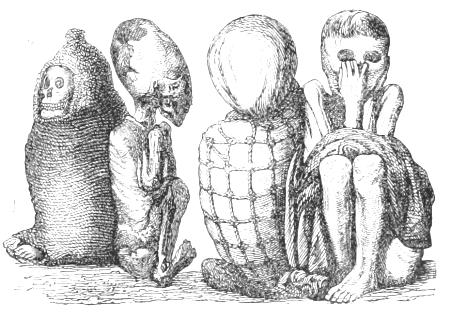
\includegraphics[scale=.5]{Fetish_or_Juju}
  \end{center}

\mybold{Supreme "Devil's" Juju; 13 Cunning; 6{,}666\AU}

\mybullet {
    \item \mybold{Ether Flute:} Playing this flute causes any Incorporeal Monster to freeze, mesmerised, so long as the user continues to play.
    \item \mybold{Golden Mule:} A tiny golden statue of a mule. Anyone carrying this doubles the number of Significant Items they can carry
    \item \mybold{Master's Ring:} This ring causes a faint tingling sensation whenever one of the wearer's employees, servants or hirelings is planning to betray them in some way.
    \item \mybold{The Displacement Doll:} Anyone attempting any Mind spell on the possessor of the Displacement Doll kind will affect only the mind of the doll. If they try to read her mind, they will read the mind of a woman trapped in a dark leather chamber, bouncing around on the body of a giant. If they try to charm her they will successfully charm the doll. 
    \item \mybold{Shrunken Head:}  Wearing the Shrunken Head on your belt gives you a +4 modifier on your \DEATH rolls
}

\OCCULT[
  Name=Damning,
  Link=occultism-damning,
  Success=9,
  Cost=666\AG
]

When you perform this ritual on a Mortal corpse no more than 7 days dead (by the law of \TheAuthority), you prevent them from departing the Isle of the Dead.  The soul is trapped in Hell permanently (though their spirit can still be lead back to the Mortal plane through \mylink{Katabasis}{occultism-katabasis}.  The corpse is consumed when this ritual is performed.


\OCCULT[
  Name=Descry,
  Link=occultism-descry,
  Success=3+,
  Cost=See below
]

You can see events transpiring within [Cunning]x100km of you by gazing into a silver bowl, censer, crystal ball, mirror, or other mystical item.  You only need to describe what you want to see and it will appear, but the vision is misty and it's hard to make out details.  You can't see things that you might not normally be able to see, so if you said you wanted to "see the body of Sir Tremalane on the northern battlefield", and the body was invisible, you might only see a bare patch of ground.  

The scrying doesn't have to only show events of the present; you can look up to [Cunning] centuries into the past.  You'd have to have a rough idea of what you'd want to see - "show me the temples of Syrinx before they were cast down" would work, but "show me the secret entrance to the Caverns of Chaos" wouldn't.  The more detailed the description of what you want to see, the better you see it.

Scrying requires that the silver bowl, censer, crystal ball be a \mylink{Minor, Major, or Greater Juju}{occultism-create-juju}.  Major Juju adds 100km and 100 years; Greater Juju adds 1,000km and 1,000 years.

  \begin{center}
  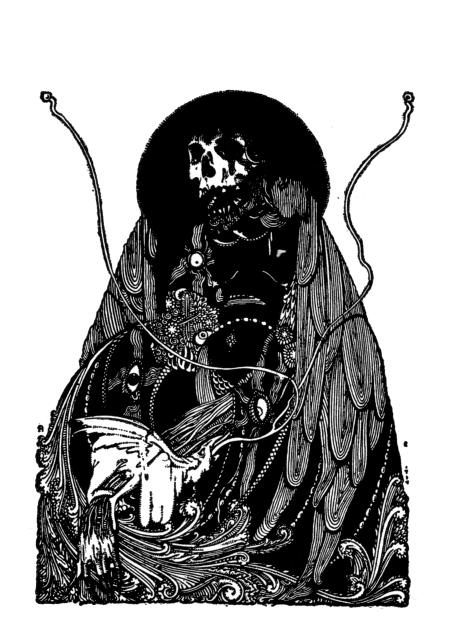
\includegraphics[scale=.5]{Occult_2}
  \end{center}



\OCCULT[
  Name=Geas,
  Link=occultism-geas,
  Success=12,
  Cost=666\AU
]

\ed{From \mybold{Places Dark \& Deep}, by the author of the blog \href{https://permacrandam.blogspot.com/}{Permanent Cranial Damage}}

You ensorcel someone with a Geas, a terrible malison that enforces an inescapable command. The command can be long and difficult, like "kill Razor the Monk" or "complete the sevenfold pilgrimage" or "bring me the Globe of the Wonder-Working King from the hoard of the Caliph Vathek" or "go away". The victim must win a \RB : \FOC contest against you.  From then on, any day that is not spent fulfilling the Geas will have one of the following effects (roll each day):

\mynumlist {
  \item Inflicted with a Curse (roll on the Curse table, re-roll any duplicates)
  \item Inflicted with a Disease (roll on the Diseases table, re-roll any duplicates)
  \item Inflicted with a Wound (roll on the Wounds table as if the target had been brough to 0 Flesh)
  \item Roll a d6: 1-3 all Tangible Stats \DCDOWN; 4-6 all Intangible Stats \DCDOWN
  \item Inability to "heal" in any way - you gain absolutely no benefits from resting
  \item Roll again - the result of the roll is inflicted on the target's loved one / parent / child / friend / etc. instead.  If the target loves nothing, the Arbiter gets to choose
}

The effect lasts until sundown; provided the subject of the Geas is "back on track", the effect ends - otherwise, roll again.

The Geas must be doable, even if it is way above the means and possibility of the victim.  Should it become impossible (following the examples above: if Razor should die in other ways, or one of the Seven Shrines be destroyed, or the Orb suddenly explode and release the 1001 demons bound inside), then the Geas is lifted.  Should you or the victim die, the Geas remains in effect, even if you are brought back from the dead or turned into undead. This spell cannot be cast on someone more than once in their lifetime.

On the upside, the Geas can empower its subject (at the Arbiter's discretion) to help them complete their task.  For example, if Razor the Monk has taken up with the King of the Merfolk, the subject of the Geas might discover they can now breathe underwater.

The target of the Geas needs to be conscious and near you when you invoke the ritual.

\OCCULT[
  Name=Haunt,
  Link=occultism-haunt,
  Success=3+,
  Cost=666\FE
]

\ed{From \mybold{Places Dark \& Deep}, by the author of the blog \href{https://permacrandam.blogspot.com/}{Permanent Cranial Damage}}

You summon [Cunning] poltergeists to haunt an Unhallowed place up to [Cunning]km away.  The poltergeists will do their best to harass and torment any Mortals who enter their domain. They can't talk and are insubstantial, but you can direct them to laugh insanely, become visible as ghostly menaces, howl discordantly, and cause telekinetic mischief, which may include the hurling of heavy or sharp objects.

\OCCULT[
  Name=Hekaphage,
  Link=occultism-hekaphage,
  Success=4+,
  Cost=varies
]

You can destroy a malison by feeding it to a Hekaphage: ethereal creatures that eat magic and Curses.  

\mybullet{
    \item a Lesser Curse requires 4 [Cunning]
    \item a Greater Curse requires 8 [Cunning]
}

Summoning a Hekaphage costs no coin (only Unhallowed Earth), but you can spend up to [Cunning]x100 coins in materials if you would like to convert coin to XP.

\cbreak

  \begin{center}
  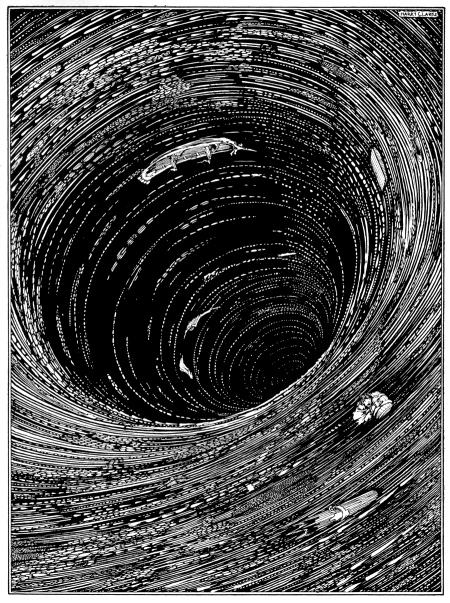
\includegraphics[scale=.5]{Occult_3}
  \end{center}



\end{multicols}

\OCCULT[
  Name=Katabasis,
  Link=occultism-katabasis,
  Success=15,
  Cost=6{,}666\AU
]

You open a way to the Isle of the Dead, where the spirits of the Hallowed dead reside for 7 days before they move on to sit at the feet of \TheAuthority (see \mylink{Damning}{occultism-damning} for keeping a spirit longer than 7 days).  The ritual must take place in a room with a single door and no windows that rests on Unhallowed Earth (or is itself Unhallowed).

By combining certain writs, components, offal, and rare ingredients, you produce 6 draughts of a potent toxin. The toxin must be ingested by willing Mortals and has no effect on unwilling participants, or the Unhallowed.  Those that ingest the poison appear to die as their \myital{noumenon} steps from their corpses.  They are now the \myital{Shikari}, the Hunters of the Dead

The \myital{Shikari} have all of their abilities and equipment that they had at the moment they died; additionally, they will find two gold coins in their mouth when they awaken in front of the door in the room. The \myital{Shikari} cannot see into the Mortal plane or interact with it in any way - there is only the door in front of them, and everything else is nothingness.

Through the door lies the Isle of the Dead.  Going through the door costs nothing, but coming back through the door costs two golden coins - they do not have to be \myital{your} coins, but you have to have two of them.  A \myital{Shikari} can never be in possession of more than 2 coins at any time.

The \myital{Shikari} can travel freely through the Isle of the Dead.  They can lead any \myital{noumenon} (soul) they find there back to the doorway (a doorway only they can see) and take them back through to the lands of the living.  They have a rough idea of where a particular Soul might be, if the Soul was known to them in the living lands. If a \myital{Shikari} dies in the Isle of the Dead, their Soul immediately departs to the feet of \TheAuthority, and they are dead forever.  

In order to pass back through the doorway, you must have two coins in your possession when you exit.  Any spirit you find in the Isle of the Dead has between 0-2 coins in their possession, depending on how they were interred by friends, family, or foes (roll a d6.  1-3: 0 coins, 4-5: 1 coins, 6: 2 coins).  There are many creatures and spirits on the Isle of the Dead (particularly crows and ravens) who try to separate the recently deceased from their coins.

If a Mortal spirit successfully exits the doorway to the Isle of the Dead, and their corpse is within the confines of the room, they may inhabit the body at no penalty (save for the likely loss of Sanity from their journey).  If the corpse is absent, the Mortal will be reincarnated - each of their Tangible Stats moves \DCDOWN (to a minimum of d3), they move to the lowest XP for their level (so if they were Level 7, they would move down to 32,000xp), and their appearance is completely different at the Arbiter's discretion.

Any who journey to the Isle of the Dead and return are forever more Unhallowed. 

\newpage

\OCCULT[
  Name=Lichdom,
  Link=occultism-lichdom,
  Success=2 (plus see below),
  Cost=66{,}666\AU
]

This dangerous and depraved rite binds a Mortal's \myital{noumenon} to a phylactery, allowing them to live on as a lich with life everlasting. In addition to the exhorbitant costs above, this rite requires:

\begin{wrapfigure}{c}{0.4\textwidth}
  \begin{center}
    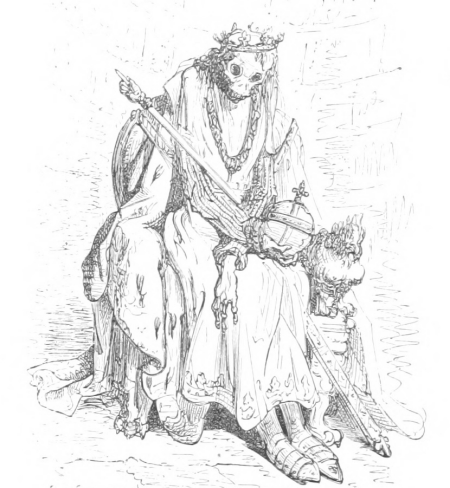
\includegraphics[scale=.5]{Lich}
  \end{center}
\end{wrapfigure}



\mylist{
    \item a phylactery (see \mylink{Create Juju}{occultism-create-juju})
    \item a dagger or knife enchanted with Bleeding (see \mylink{Sword Magic}{spriggan-sword-magic})
    \item a Mortal vessel - that is, a human corpse - dead for less than 7 days
}



The witch performing the ritual must do the following:

\mynumlist {
    \item The soon-to-be-Lich, witch, coven, and \myital{Shikari} must all be in a room suitable for the ritual of \mylink{Katabasis}{occultism-katabasis}.
    \item The phylactery is given to the Mortal who wishes to become a lich.  The Mortal is then stabbed with the enchanted dagger, and their blood used to wash the relic. 
    \item A Leech must use Mend to keep the Mortal alive as long as possible.  Every time the Bleeding is staunched, the lich must be stabbed again.
    \item Once the Mortal dies, the ritual of \mylink{Damning}{occultism-damning} must be performed, which will consume the corpse
    \item The ritual of \mylink{Katabasis}{occultism-katabasis} must then be performed; however, the ritual produces \mybold{no coins}, as the magic used to create the coins must instead be used to profane the phylactery so that it might be carried by the dead who have drunk the poison.  Anyone who wants to come back will need to find some coins on the other side, including 2 for the Mortal attempting to become a Lich
    \item Trusted minions must now carry the phylactery into the Isle of the Dead, find the soul of the lich, and coax it into the phylactery.  The \myital{noumenon} of the Lich will now be inside of the phylactery forever more.  They cannot die so long as the phylactery remains intact.
}

Once the \myital{Shikari} and the lich return, the lich is reincarnated in a vessel that is in all ways their original self, with no loss of power or skill, though they will appear cadaverous. Despite this, they now only age 1 year for every 1,000 years that pass; they are immune to iron weapons, Toxins, and spells of the Mind and Entropy paradigms; they may commit as many spells as they desire to be inscribed inside their skulls (making Lich skulls extremely potent magical books in their own right); and they are able to read and speak all languages



\begin{multicols}{2}\raggedcolumns

\OCCULT[
  Name=Malison,
  Link=occultism-malison,
  Success=3+,
  Cost=See below
]

You can place one of the base {Curses}{table-curses}:

\mylist {
  \item on a person within [Cunning]km; 
  \item on an item; or 
  \item on your familiar.  
}

\mybullet{
    \item a \myital{random} Lesser Curse requires 3 [Cunning]
    \item a \myital{specific} Lesser Curse requires 5 [Cunning]
    \item a \myital{random} Greater Curse requires 7 [Cunning]
    \item a \myital{specific} Greater Curse requires 9 [Cunning]

}


If the curse is chosen randomly, at least 3 [Cunning] is required.  If you wish to choose the curse, at least 6 [Cunning] is required.  The more Cunning you use, the more difficult it will be to remove the curse with \mylink{Hekaphage}{occultism-hekaphage}.

You can break any of your own curses at will. Malisons survive the death of the witch that casts them.  The cost to cast the curse is [Cunning]x10\AU


\OCCULT[
  Name=Unhallowed Earth,
  Link=occultism-unhallowed-earth,
  Success=2+ (plus see below),
  Cost=66\AU
]

You can either desecrate Hallowed Ground, or create Unhallowed Earth for the casting of rituals, somewhere within [Cunning]km of you.  You create / desecrate an area [Cunning]x2 meters in diameter.  If you're attempting to desecrate Hallowed Ground, the diameter must be equal to or exceed the area of the Hallowed Ground.  You must create a \mylink{Witch Mark}{occultism-witch-mark} that will be consumed during the ritual; this Witch Mark identifies the Unhallowed Earth as "belonging" to you.  Another Mystic knows the size of the Unhallowed Earth, but not necessarily who it belongs to.

Unhallowed Earth with your Witch Mark on it provides the following benefits:

\mybullet {
  \item no Mortals may enter Unhallowed Earth unless you accompany them
  \item you may immediately end a Markovian effect while standing on the Unhallowed Earth
  \item you may ignore the negative effect of a Failure when using your Mojo (that is, you may keep your Mojo die even if they roll a 1 or a 2) while standing on the Unhallowed Earth
  \item finally, no Sacraments may be performed on Unhallowed Earth
}

This ritual is the only one that does \mybold{not} require Unhallowed Earth to perform. 



\OCCULT[
  Name=Witch Mark,
  Link=occultism-witch-mark,
  Success=2,
  Cost=66\AG
]

A personal mark of power placed on any non-living item.  The mark itself is not magical, but requires the \mylink{Third Eye}{charm-third-eye} to see. Unless you've seen this Witch Mark before (if you knew the Mystic personally, for example), a Skill: Lore check is required to determine the owner of the Witch Mark.  Unhallowed Earth imbued with your Witch Mark follows the same rules (visible via the Third Eye, requires a Skill:Lore check to identify the owner).


}%end
